\begin{recipe}{松子肉}

\ingredients

\ingredient{豆油皮}{一张}
\ingredient{萝卜}{四两五}
\ingredient{猪肉}{二两}
\ingredient{鸡蛋}{二个}
\ingredient{胡椒}{三分}
\ingredient{菜油}{一斤耗一两五}
\ingredient{干豆粉}{三钱}
\ingredient{奶汤}{四两}
\ingredient{二汤}{二两}
\ingredient{盐}{五分}
\ingredient{味精}{二分}
\ingredient{松子}{二钱}
\ingredient{葱}{二钱}
\ingredient{姜}{六分}

\preparation

\step 选用肥瘦相连的猪肉,洗净,切成二寸长、一分半厚的细丝。松子去皮捶茸放于肉
丝中。萝卜去皮,切成二分厚、二寸长的粗丝,挤干水。姜、葱均切成细丝。

\step 鸡蛋去壳与干豆粉调匀成为蛋清豆粉,加入味精、盐、
\begin{wrapfigure}[7]{l}{17em}%
\vspace{-1.125\baselineskip}%
\begin{center}%
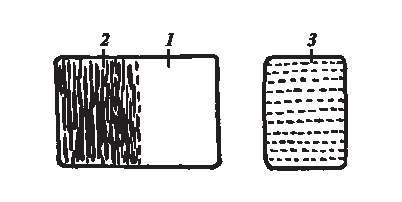
\includegraphics[scale=1]{illustration-003.eps}%
\vspace{-.55\baselineskip}%
\caption{松子肉包叠法图}%
\label{pine nut meat wrapping method}%
{\small 1. 豆油皮 2. 肉丝 3. 叠好后}%
\end{center}%
\end{wrapfigure}%
胡椒,于深碗中混合好,再与猪肉丝、萝卜丝、姜、葱一并拌匀。


\step 豆油皮一张修成六寸宽、八寸长,平铺案板上,而后把拌匀的猪肉丝、萝卜丝等铺
在豆油皮上,铺成七分厚,铺上豆油皮的一半,再把另一半叠过来,接头处涂蛋淸豆粉封
口,如图~\ref{pine nut meat wrapping method}\,。

\step 炒锅倒入菜油烧红,将叠好的豆油皮包放入炸透,炸成金黄色,泌去炸油,放盘中
晾冷。再用刀切成一寸半长、
\begin{wrapfigure}[5]{l}{10em}%
\vspace{-1.9\baselineskip}%
\begin{center}%

\includegraphics[scale=1]{illustration-004.eps}%
\vspace{-.55\baselineskip}%
\caption{松子肉摆法}%
\label{pine nut meat plate presentation}%
\end{center}%
\end{wrapfigure}%
三分宽、七分厚的长条,共二十四条。以六条为一组,于碗中镶成卍字形,如
图~\ref{pine nut meat plate presentation}\,。然后加二汤淹没肉条,上笼蒸三十分钟
取出,扣于碗内,再加奶汤四两、盐七分即成。


\features

此菜香软可口,营养丰富,特别适于冬季食用。

\end{recipe}

% vim: filetype=tex noautoindent nojoinspaces
% vim: fileencoding=utf-8 formatoptions+=m
% vim: textwidth=78 tabstop=4 shiftwidth=4 softtabstop=4
